\mySection{Ingreso al sistema (\textit{login}) y cambio de contraseña}
En esta sección explicamos cómo ingresar al sistema y cómo cambiar la contraseña.

\mySubSection{Ingreso al sistema (\textit{login})}
La primer pantalla que vemos al ingresar a la aplicación es la de \textit{login} (figura \ref{fig:login}).
\begin{figure}
\centerline{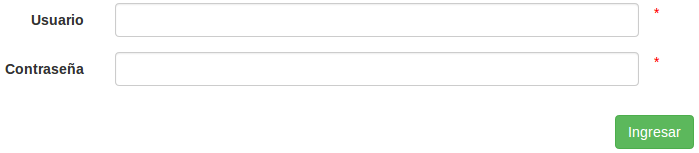
\includegraphics[width=0.7\textwidth]{login.png}}
\caption{Pantalla de ingreso al sistema}
\label{fig:login}
\end{figure}
Allí debemos ingresar correctamente el usuario y la contraseña. Si ingresamos mal alguno de los campos no podremos ingresar al sistema y se nos muestra un mensaje de error (figura \ref{fig:login_fallido}).
\begin{figure}
\centerline{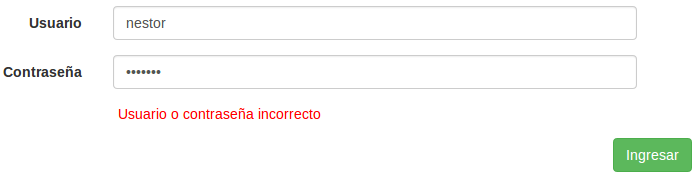
\includegraphics[width=0.7\textwidth]{login_fallido.png}}
\caption{Login fallido}
\label{fig:login_fallido}
\end{figure}

\mySubSection{Cambio de contraseña}\label{cap:cambio_pass}
Para acceder a la pantalla de cambio de contraseña nos dirigimos hacia el nombre del usuario actual y luego a ``Cambiar contraseña'' (ver figura \ref{fig:menu_cambio_pass}).
\begin{figure}
\centerline{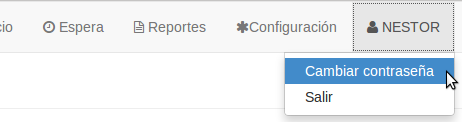
\includegraphics[width=0.7\textwidth]{menu_cambio_pass.png}}
\caption{Menú de cambio de contraseña}
\label{fig:menu_cambio_pass}
\end{figure}
Allí debemos ingresar la contraseña actual y la nueva (dos veces) (figura \ref{fig:cambio_pass}).
\begin{figure}
\centerline{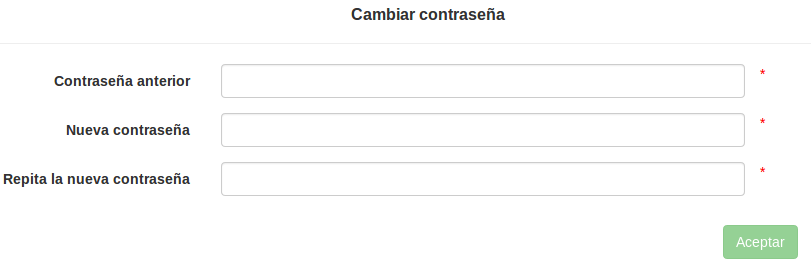
\includegraphics[width=0.7\textwidth]{cambio_pass.png}}
\caption{Cambio de contraseña}
\label{fig:cambio_pass}
\end{figure}
Validaciones a tener en cuenta:

\begin{itemize}
\item El nombre del usuario debe tener al menos tres caracteres.
\item La contraseña debe tener al menos 4 caracteres.
\item Para la contraseña el sistema distingue entre mayúsculas y minúsculas. Si, por ejemplo, nuestra contraseña es ``Clave'' y en la pantalla de \textit{login} ingresamos ``clave'', no podremos ingresar al sistema.
\item Siempre que se crea un usuario nuevo la contraseña por default es ``triage'' (se recomienda cambiar la misma por una clave secreta en el primer acceso al sistema).
\end{itemize}